\documentclass{article}%
\usepackage[T1]{fontenc}%
\usepackage[utf8]{inputenc}%
\usepackage{lmodern}%
\usepackage{textcomp}%
\usepackage{lastpage}%
\usepackage{authblk}%
\usepackage{graphicx}%
%
\title{Inhibition of rhabdomyosarcoma cell and tumor growth by targeting specificity protein (Sp) transcription factors}%
\author{Sarah Diaz}%
\affil{CAS Key Laboratory of Pathogenic Microbiology and Immunology, Institute of Microbiology, Chinese Academy of Sciences, Beijing, China}%
\date{01{-}01{-}2009}%
%
\begin{document}%
\normalsize%
\maketitle%
\section{Abstract}%
\label{sec:Abstract}%
A study published Dec. 5 in Nature Genetics suggests that different types of immune cells control how insulin fails to work properly in human kidneys.\newline%
"The best analogy might be children," said lead author Benjamin Bialosky, assistant professor in the department of medicine at USC. "In a child, blood sugar levels are high and the immunosuppressant cells in the brain create a model immune response. At the same time, the more body weight the child is carrying, the less sensitive the immune system is to any rejection."\newline%
The mice model diabetes developed the following characteristics: Children's immune cells seem to display antibodies that can neutralize insulin and food.\newline%
In general, adults who have type 1 diabetes develop high levels of the most well{-}known inflammatory response, known as interleukin{-}1beta (IL{-}1 beta). In people with type 2 diabetes, which involves more of a tissue{-}based immune response, new immunological profiles are developed at different stages of the disease.\newline%
In Bialosky's research, immune{-}protection immune cells known as hemagglutinin (HA) cells (led by "ME) cells were tested on mice lacking blood sugar{-}regulating antigens. The mice were genetically engineered to have low HA levels and researchers fed them corn gluten instead of healthy food, known as soy.\newline%
As a result, they had low levels of HA. Additionally, they showed reduced protein production.\newline%
The researchers found that HA cells which normally respond to insulin resistance exhibited a rapidly reduced output, thereby producing a blanket immune response that weakened the blood sugar defenses of the mice.\newline%
The results are significant because they show that antibodies to HA cells, known as antigen{-}presenting cells (APCs), could suppress blood sugar responses in patients with diabetic nephropathy, Bialosky said.\newline%
Additionally, HA cells are now proliferating in these mice and tumors in the kidneys might be caused by ethanol{-}induced neuropathy, or nerve injury, as a result of antigens blocking glucose metabolism in this region of the brain.

%
\subsection{Image Analysis}%
\label{subsec:ImageAnalysis}%


\begin{figure}[h!]%
\centering%
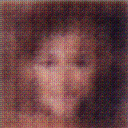
\includegraphics[width=150px]{500_fake_images/samples_5_424.png}%
\caption{A Close Up Of A Person Holding A Cell Phone}%
\end{figure}

%
\end{document}